%\appendix{Представление графического материала}

Графический материал, выполненный на отдельных листах,
изображен на рисунках А.1--А.\arabic{числоПлакатов}.
\setcounter{числоПлакатов}{0}

\renewcommand{\thefigure}{А.\arabic{figure}} % шаблон номера для плакатов

\begin{landscape}

\begin{плакат}
    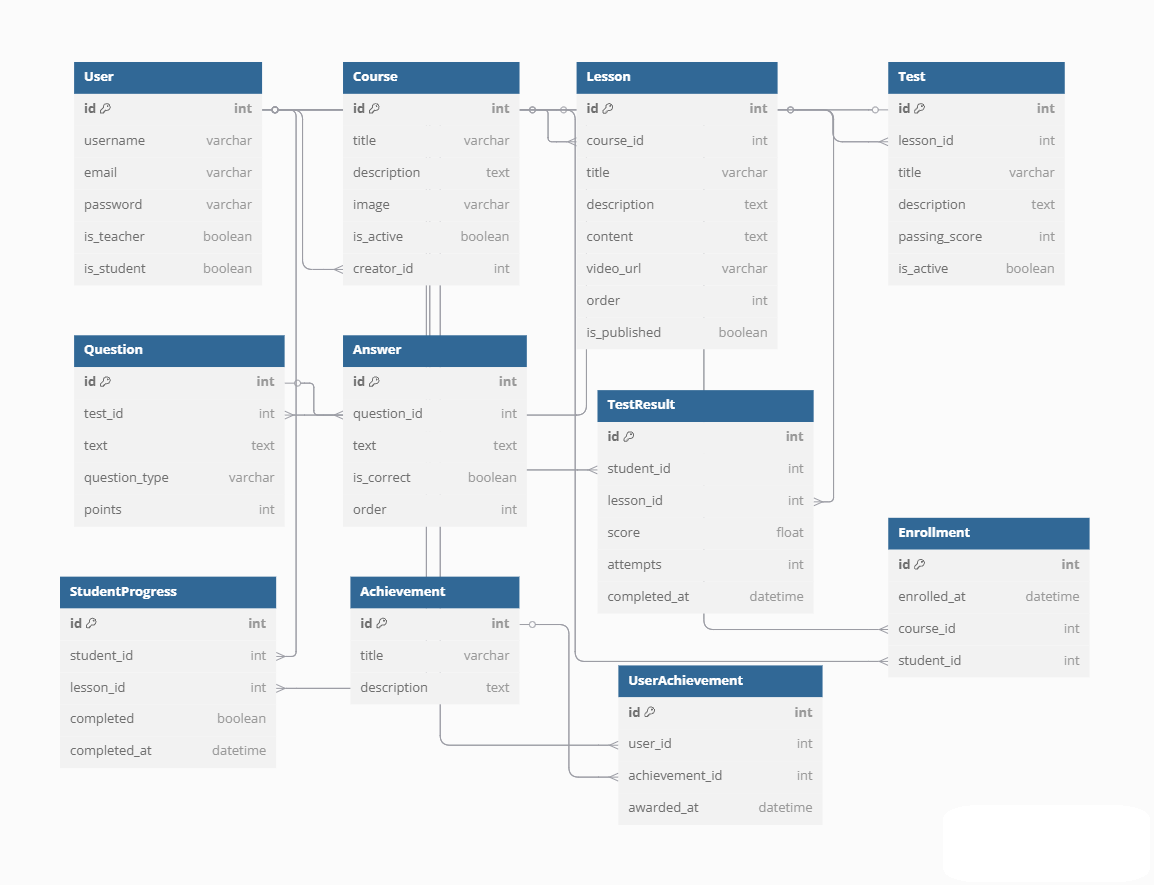
\includegraphics[width=1\linewidth]{бд}
    \заголовок{Сведения о ВКРБ}
    \label{pl1:image}      
\end{плакат}

\begin{плакат}
    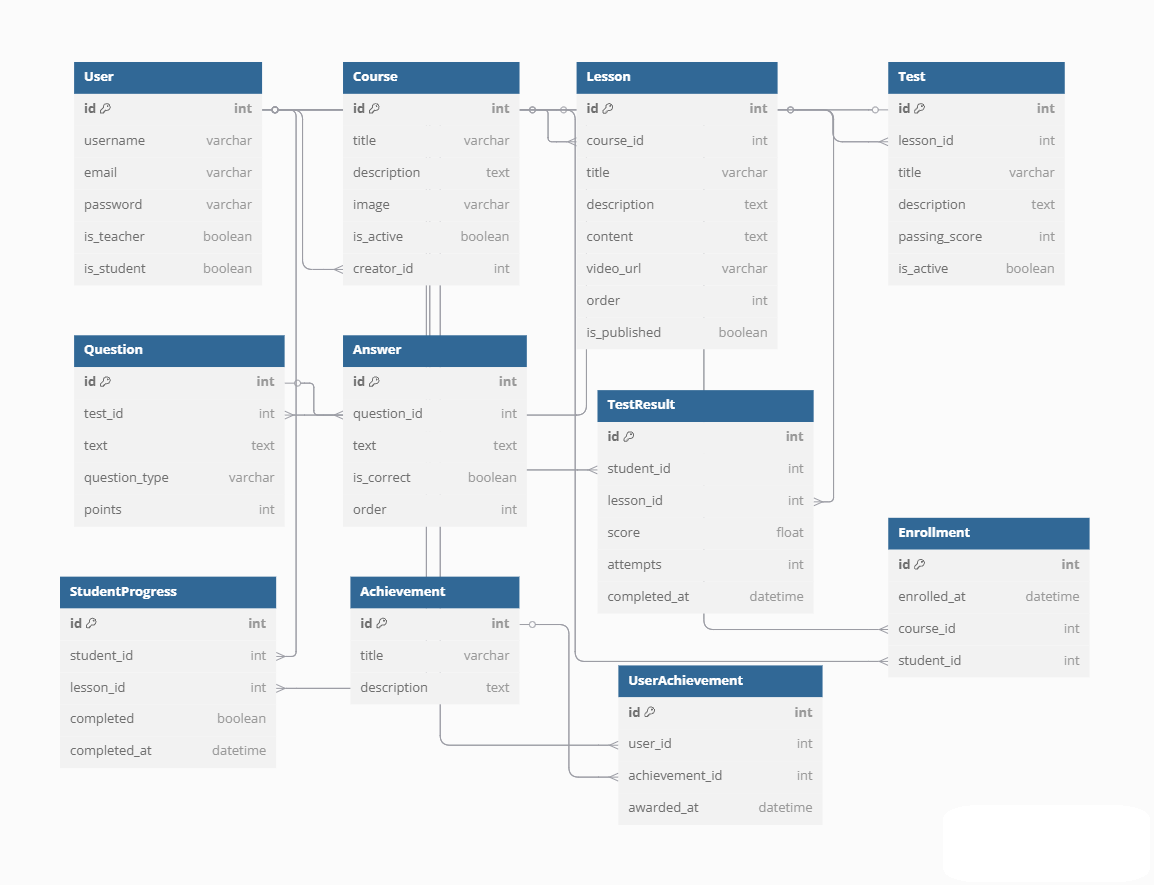
\includegraphics[width=1\linewidth]{бд}
    \заголовок{Цель и задачи разработки}
    \label{pl2:image}      
\end{плакат}

\begin{плакат}
    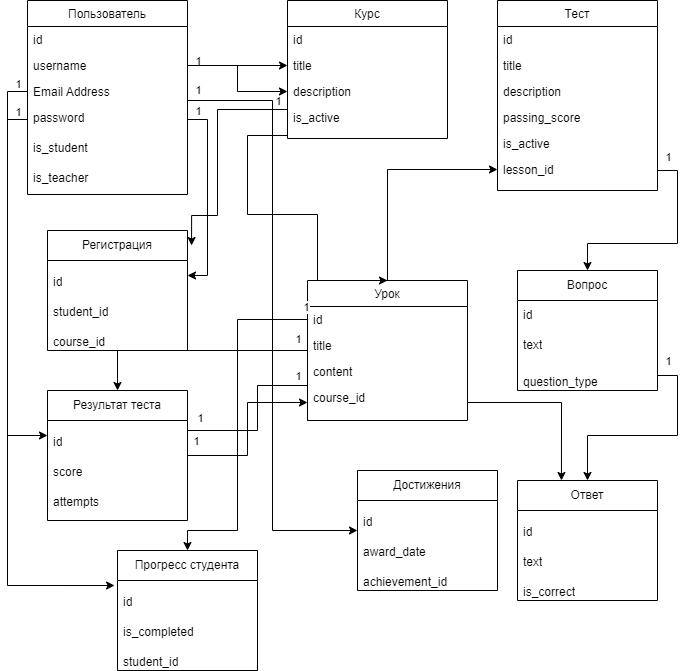
\includegraphics[width=0.7\linewidth]{концептуальная}
    \заголовок{Концептуальная модель сайта}
    \label{pl3:image}      
\end{плакат}

\begin{плакат}
    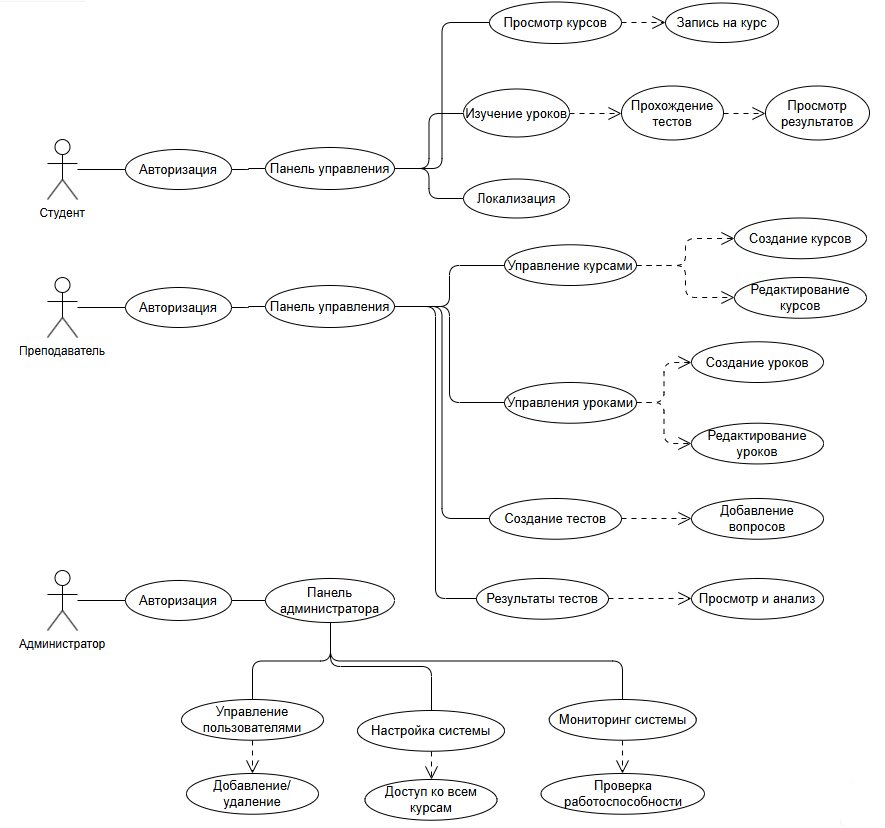
\includegraphics[width=0.7\linewidth]{UML}
    \заголовок{Диаграмма прецедентов}
    \label{pl4:image}      
\end{плакат}

\begin{плакат}
	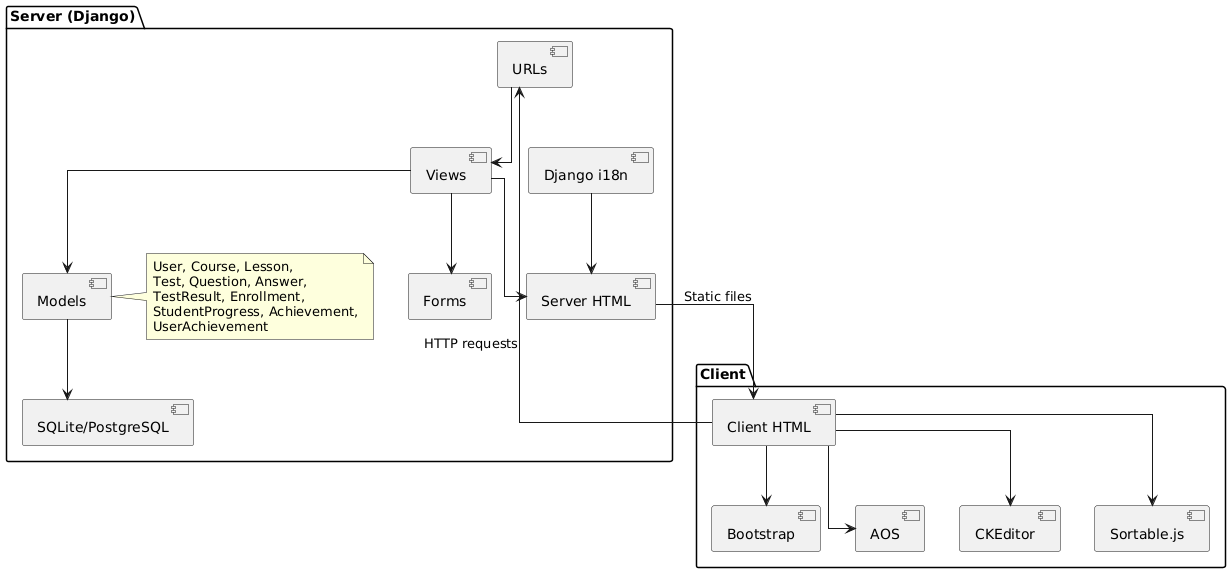
\includegraphics[width=0.7\linewidth]{диаграмма1}
	\заголовок{Диаграмма компонентов}
	\label{pl5:image}      
\end{плакат}

\end{landscape}
